\documentclass[tikz,border=0pt]{standalone}
\usepackage[T1]{fontenc}
\usepackage{helvet}
\usetikzlibrary{arrows.meta}
\renewcommand{\familydefault}{\sfdefault}
\definecolor{navy}{HTML}{123B61}
\definecolor{teal}{HTML}{146B6B}
\definecolor{slate}{HTML}{575F63}
\definecolor{lightgray}{HTML}{EDF0F1}
\definecolor{ink}{HTML}{182B34}
\definecolor{rulegray}{HTML}{54636A}
\newcommand{\bodytype}{\fontsize{8.3}{10.2}\selectfont}
\newcommand{\headtype}{\bfseries\fontsize{10.4}{12}\selectfont}
\newcommand{\rowtype}{\bfseries\fontsize{8.1}{10}\selectfont}
\begin{document}
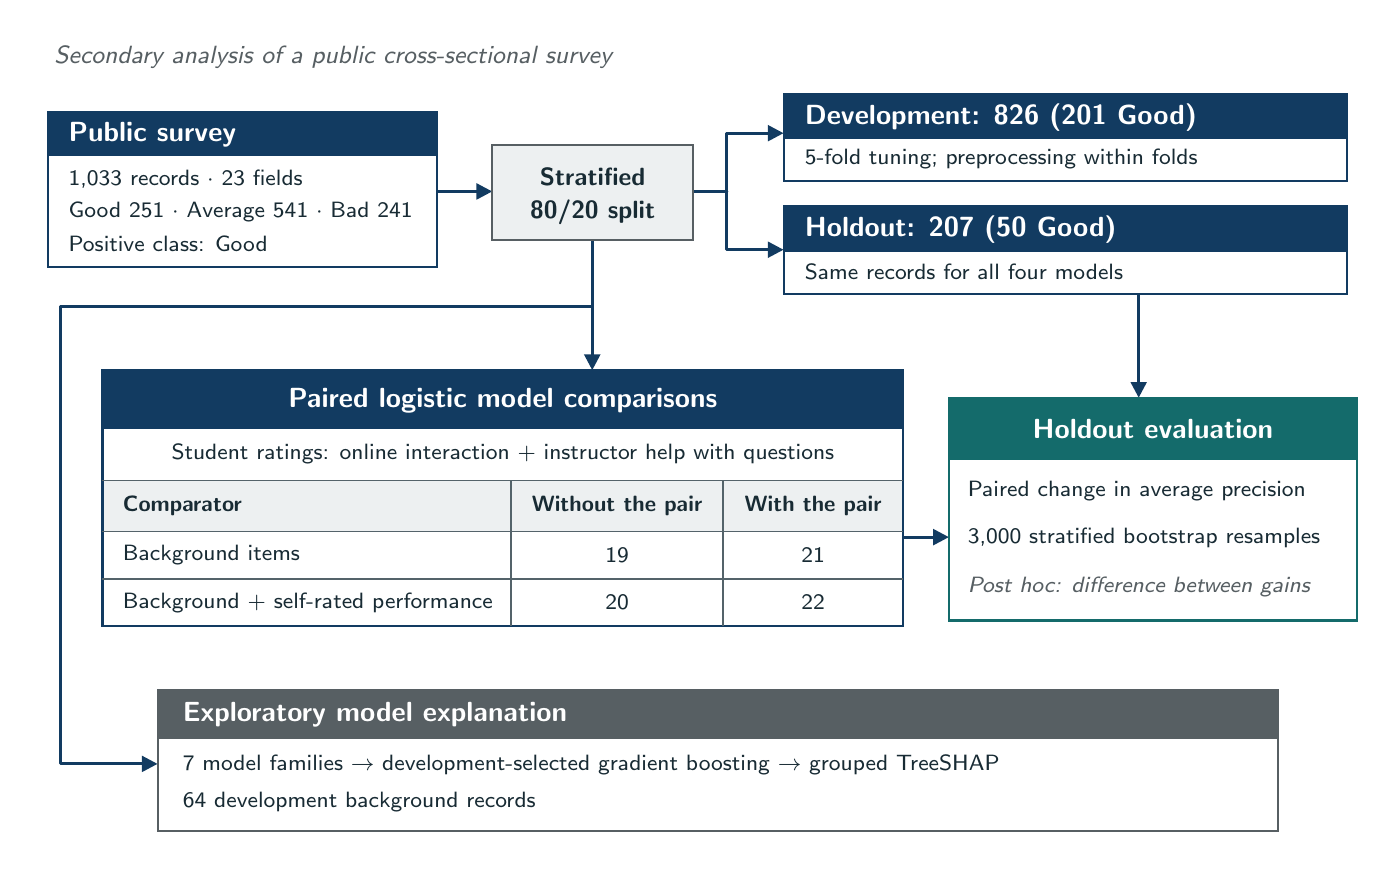
\begin{tikzpicture}[x=1mm,y=-1mm,
  every node/.style={inner sep=0pt,outer sep=0pt,text=ink,font=\bodytype},
  flow/.style={draw=navy,line width=1.05pt,-{Triangle[length=2mm,width=2mm]},line cap=round,line join=round},
  branch/.style={draw=navy,line width=1.05pt,line cap=round,line join=round},
  head/.style={text=white,font=\headtype},
  rule/.style={draw=rulegray,line width=.48pt}]
\path[use as bounding box] (0,0) rectangle (170,105);
\fill[white] (0,0) rectangle (170,105);
\node[anchor=west,text=slate,font=\itshape\fontsize{9.1}{11}\selectfont] at (3.4,3.8) {Secondary analysis of a public cross-sectional survey};

\draw[flow] (52,20.8) -- (59,20.8);
\draw[branch] (84.5,20.8) -- (88.8,20.8);
\draw[flow] (88.8,20.8) |- (96.0,13.4);
\draw[flow] (88.8,20.8) |- (96.0,28.2);
\draw[flow] (71.7,27) -- (71.7,43.5);
\draw[flow] (71.7,35.4) -- (4.2,35.4) -- (4.2,93.5) -- (16.5,93.5);
\draw[flow] (141.1,33.8) -- (141.1,47);
\draw[flow] (111.2,64.7) -- (117,64.7);

\draw[fill=white,draw=navy,line width=.78pt] (2.6,10.7) rectangle (52,30.4);
\fill[navy] (2.6,10.7) rectangle (52,16.3);
\node[head,anchor=west] at (5.2,13.55) {Public survey};
\node[anchor=west] at (5.2,19.2) {1,033 records $\cdot$ 23 fields};
\node[anchor=west] at (5.2,23.4) {Good 251 $\cdot$ Average 541 $\cdot$ Bad 241};
\node[anchor=west] at (5.2,27.5) {Positive class: Good};

\draw[fill=lightgray,draw=slate,line width=.72pt] (59,14.9) rectangle (84.5,27);
\node[font=\bfseries\fontsize{9.2}{11}\selectfont] at (71.75,18.9) {Stratified};
\node[font=\bfseries\fontsize{9.2}{11}\selectfont] at (71.75,23.5) {80/20 split};

\draw[fill=white,draw=navy,line width=.78pt] (96,8.45) rectangle (167.6,19.5);
\fill[navy] (96,8.45) rectangle (167.6,14.2);
\node[head,anchor=west] at (98.7,11.4) {Development: 826 (201 Good)};
\node[anchor=west] at (98.7,16.65) {5-fold tuning; preprocessing within folds};
\draw[fill=white,draw=navy,line width=.78pt] (96,22.7) rectangle (167.6,33.8);
\fill[navy] (96,22.7) rectangle (167.6,28.45);
\node[head,anchor=west] at (98.7,25.65) {Holdout: 207 (50 Good)};
\node[anchor=west] at (98.7,31.05) {Same records for all four models};

\draw[fill=white,draw=navy,line width=.8pt] (9.5,43.5) rectangle (111.2,76.0);
\fill[navy] (9.5,43.5) rectangle (111.2,51.0);
\node[head] at (60.35,47.3) {Paired logistic model comparisons};
\node at (60.35,54.2) {Student ratings: online interaction + instructor help with questions};
\fill[lightgray] (9.65,57.5) rectangle (111.05,64.0);
\draw[rule] (9.5,57.5) -- (111.2,57.5)
 (9.5,64.0) -- (111.2,64.0)
 (9.5,70.0) -- (111.2,70.0)
 (61.4,57.5) -- (61.4,76.0)
 (88.3,57.5) -- (88.3,76.0);
\node[anchor=west,font=\rowtype] at (12.1,60.8) {Comparator};
\node[font=\rowtype] at (74.85,60.8) {Without the pair};
\node[font=\rowtype] at (99.75,60.8) {With the pair};
\node[anchor=west] at (12.1,67.0) {Background items};
\node[anchor=west] at (12.1,73.0) {Background + self-rated performance};
\node at (74.85,67.0) {19};
\node at (99.75,67.0) {21};
\node at (74.85,73.0) {20};
\node at (99.75,73.0) {22};

\draw[fill=white,draw=teal,line width=.85pt] (117,47) rectangle (168.8,75.3);
\fill[teal] (117,47) rectangle (168.8,54.9);
\node[head] at (142.9,51.0) {Holdout evaluation};
\node[anchor=west] at (119.4,58.8) {Paired change in average precision};
\node[anchor=west] at (119.4,64.8) {3,000 stratified bootstrap resamples};
\node[anchor=west,text=slate,font=\itshape\bodytype] at (119.4,71) {Post hoc: difference between gains};

\draw[fill=white,draw=slate,line width=.78pt] (16.5,84.1) rectangle (158.8,102.05);
\fill[slate] (16.5,84.1) rectangle (158.8,90.35);
\node[head,anchor=west] at (19.7,87.25) {Exploratory model explanation};
\node[anchor=west] at (19.7,93.65) {7 model families $\rightarrow$ development-selected gradient boosting $\rightarrow$ grouped TreeSHAP};
\node[anchor=west] at (19.7,98.35) {64 development background records};
\end{tikzpicture}
\end{document}
